\subsection{Aufbau und praktisch Relevantes}
\begin{figure}[h!]
	\centering
	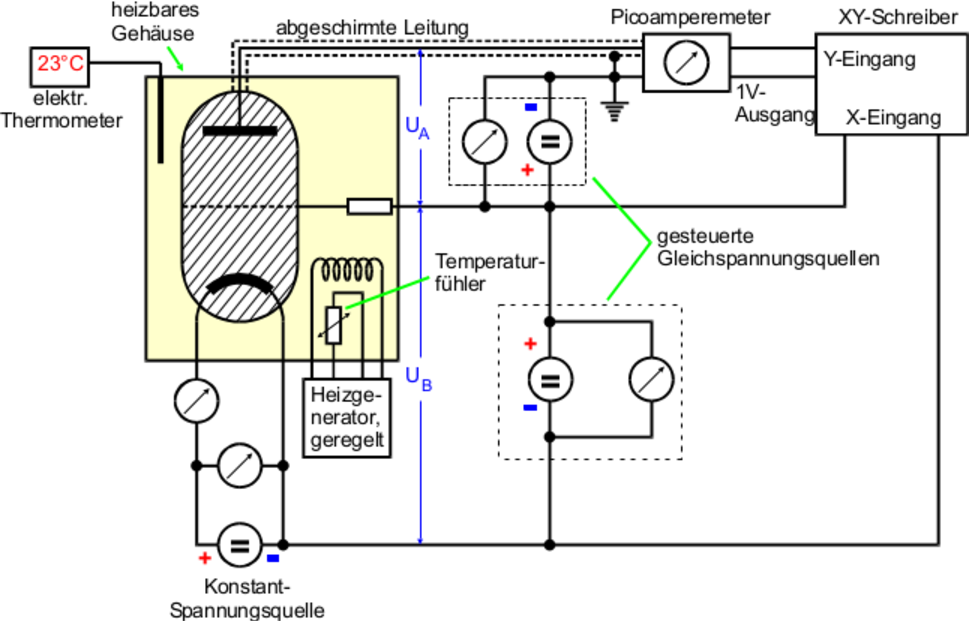
\includegraphics[width = 0.85\textwidth]{Aufbau_Schaltbild.pdf}
	\caption{Schaltbild zum Versuch \cite{\V}}
	\label{fig:Schaltbild}
\end{figure}
\todo{Ich würde ihn gerne fragen, was passiert, wenn $U_A$ negativ wird. Weil dann legt $U_A$ an der Beschleungigungselektrode eine negative Spannung an und $U_B$ eine positive. Gibts da nicht irgendwie nen Kurzschluss oder so? Oder hebt sich das wirklich einfach so auf?}

Abbildung \ref{fig:Schaltbild} zeigt den verwendeten Versuchsaufbau. Gelb hinterlegt ist der im vorigen Kapitel beschriebene eigentliche Aufbau. Beim tatsächlichen Aufbau im Labor und den damit zu erwartenden Ergebnissen sind allerdings weitere Punkte zu beachten:
\subsubsection*{Dampfdruck}
Der Dampfdruck im Glaskolben muss kontrolliert werden. Ist er zu gering, sind die \ce{Hg}-Atome zu weit von einander entfernt. Dann würden die Elektronen ohne Stoß bis zur Beschleunigungselektrode kommen, selbst wenn ihre Energie für eine Anregung der Atome ausreichend ist. Ist er zu hoch, liegen die Atome so dicht beieinander, dass die Elektronen sehr häufig elastische Stöße ausführen (und ihre Richtung ändern), was dafür sorgt, dass weniger Elektronen an der Beschleunigungselektrode ankommen. Für die mittlere Weglänge $w$ in \si{\centi\meter} zwischen den Atomen gilt
\begin{align}\label{eq:weglange}
	w = \frac{2.9}{p_\text{sät}} \ ,
\end{align}
wobei $p_\text{sät}$ der Sättigungsdampfdruck in \si{\bar} ist. Für den Dampfdruck gilt
\begin{align}\label{eq:dampfdruck}
	p(T) = \SI{5.5e7}\exp\left(-\frac{6876}{T}\right) \ ,
\end{align}
er kann also einfach über die Temperatur $T$ im Gefäß reguliert werden.
\subsubsection*{Kontaktpotential}
Haben die zwei Elektroden einer Spannungsquelle unterschiedliche Austrittsarbeiten, weicht die real anliegende Spannung von der am Gerät eingestellten ab. Dieses Problem tritt bei der Beschleunigungsspannung auf, denn der Glühdraht sollte aus einem Material sein, dessen Austrittsarbeit $\Phi_\text{G}$ sehr gering ist. Die Beschleunigungselektrode dagegen hat eine vergleichsweise hohe Austrittsarbeit $\Phi_\text{B}$. Mit Abbildung \ref{fig:Kontakt} gilt
\begin{align}
	U_\text{B,eff} = U_\text{B} - \underbrace{\frac{\Phi_\text{B}-\Phi_\text{G}}{e}}_{:=K} \ ,
\end{align}
mit dem Kontaktpotential $K$. Die später aufgenommenen Kurven sind demnach um $K$ verschoben.
\begin{figure}[h!]
	\centering
	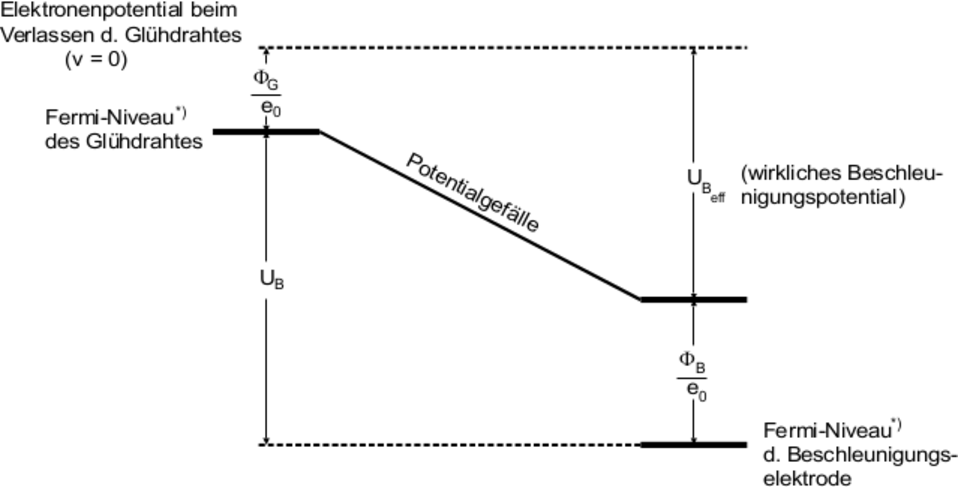
\includegraphics[width = 0.8\textwidth]{Kontaktpot.pdf}
	\caption{Veranschaulichung der Zusammenhänge zwischen Austrittsarbeiten und Beschleunigungsspannung \cite{\V}}
	\label{fig:Kontakt}
\end{figure}
\todo{Warum wird $\Phi_B$ dann nicht auch sehr klein gewählt? Weil da sonst auch Elektronen rauskämen?}
\subsubsection*{Energie-Spektrum der Elektronen}
Idealisiert wird davon ausgegangen, dass die Elektronen nach direkt nach dem Auslösen aus dem Glühdraht alle eine kinetische Energie von $E_\text{kin} = 0$ haben. In Wirklichkeit aber besitzen die Elektronen schon im Metall unterschiedliche Energien. Sie werden durch die Fermi-Dirac-Verteilung beschrieben, sie beschreibt die Häufigkeit in Abhängigkeit von der Energie. Elektronen mit sehr geringer Energie im Metall kommen sehr häufig vor, die Häufigkeit fällt mit zunehmender Energie sehr schnell ab. Diese kontinuierliche Energieverteilung sorgt dafür, dass die später gemessenen Pieks nicht so steil abfallen, wie aus der Theorie erwartet.

\clearpage

\subsection{Messung}
Die Messung besteht aus der Aufzeichnung verschiedener Kurven mit dem XY-Schreiber. \\
Die erste Kurve ist $I_\text{A}(U_\text{A})$. Sie wird bei konstanter Beschleunigungsspannung
\begin{align}
	U_\text{B} = \SI{11}{\volt}
\end{align}
und jeweils einmal bei einer Temperatur von $T=\SI{25}{\celsius}$ und $T=\SI{130}{\celsius}$ aufgenommen. \\
Dann wird die Franck-Hertz-Kurve $I_\text{A}(U_\text{B})$, mit konstanter Bremsspannung
\begin{align}
	U_\text{A} = \SI{1}{\volt}
\end{align}
bei einer Temperatur von $T = \SI{100}{\celsius}$. \\
Zuletzt wird zur Bestimmung der Ionisierungsenergie eine (nun beschleunigende) Spannung
\begin{align}
	U_\text{A} = \SI{-30}{\volt}
\end{align}
angelegt und wieder $I_\text{A}(U_\text{B})$ aufgetragen.